
\section{Literature Review of droplet impacts}

Droplet impact has been investigated from more than a century.These studies can be classified into three broad categories :- 
\begin{enumerate}
 \item Experimental Phenomenology.
 \item Simulation.
 \item Theory.
\end{enumerate}

There are many studies which are combination of the two or more as well e.g. \cite{Mao1997} has proposed theoretical models which were supported by experiments. We
begin with a brief discussion on experimental phenomenology.
\subsection{Experimental Phenomenology}
With the advent of high speed photography in late 1800s, it became possible to observe numerous phenomena which were too fast for the human eye.
Having developed the skills of high speed photography, \cite{Worthington1908} captured photographs of droplet impact. Since then various aspects of
droplet impact have being studied. There are now sophisticated digital systems which can record images at a very high frame rate 
(See Figure \ref{gunjal}) that enable us to capture very fast dynamics which are not visible to human eye.
\begin{figure}[tbp]
\centering
 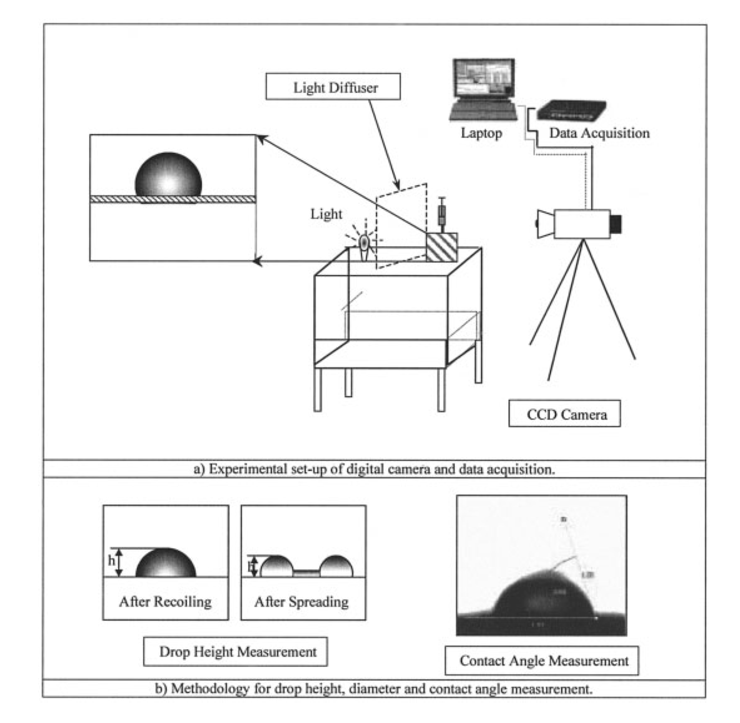
\includegraphics{gunjal.eps}
 \caption[Experimental setup to study droplet impact]{Experimental setup to study droplet impact by \cite{Gunjal2005}}
 \label{gunjal}
\end{figure}
\cite{Richard2000} observed for impact on highly hydrophobic surface (contact angle $ > 170^o$), droplets fully bounce, they 
do not tend to spread (See Figure \ref{richard}). They behaved just like spring but found there was a limit in elasticity due to the transfer
of the part of kinetic energy into the drop vibrations.
\begin{figure}[tbp]
\centering
 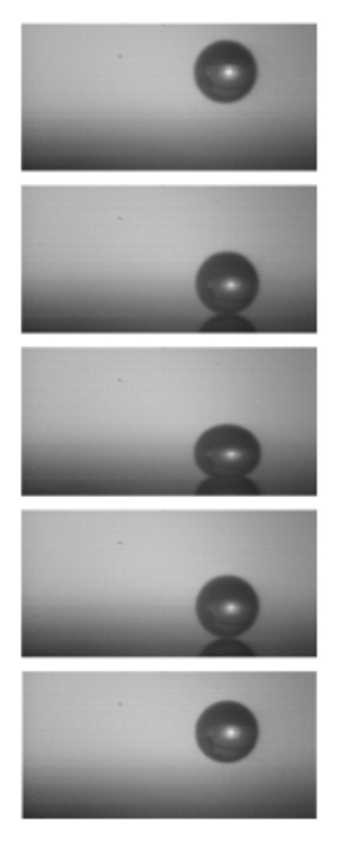
\includegraphics{richard.eps}
 \caption[Droplet impact on superhydrophobic surface]{Droplet impact(R = 0.4 mm) on superhydrophobic surface
 by \cite{Richard2000} }
 \label{richard}
\end{figure}
Droplet impact on dry surfaces are quite different when compared to wet surfaces. \cite{Rioboo2001} studied the effect
various flow parameters and surface characteristics on the droplet impact dynamics. They discovered six different outcomes of a droplet impact on 
a dry surface. In Figure \ref{rioboo} they explained the deposition as droplet deformation and continuous attachment to the surface while spreading without breakup. When
the droplet impacted with a rough surface a splash initiated in the direction of contact line velocity at the onset of spreading called as prompt splash.
Another kind of splash can be seen above the solid surface at the rim of a corona and generally referred to as corona splash.
Sometimes a breakup can be seen while the droplet is receding after maximum spreading, this is attributed to the fact while receding the dynamic contact angle decreases and when 
the limiting value is reached some drops are left behind by the receding lamella. It looks beautiful when a droplet rebounds, this particular process occurs only when a
receding phase  precedes. A full rebound occurs when the dynamic contact angle is large and the receding phases are high in kinetic energy.
\begin{figure}[tbp]
\centering
 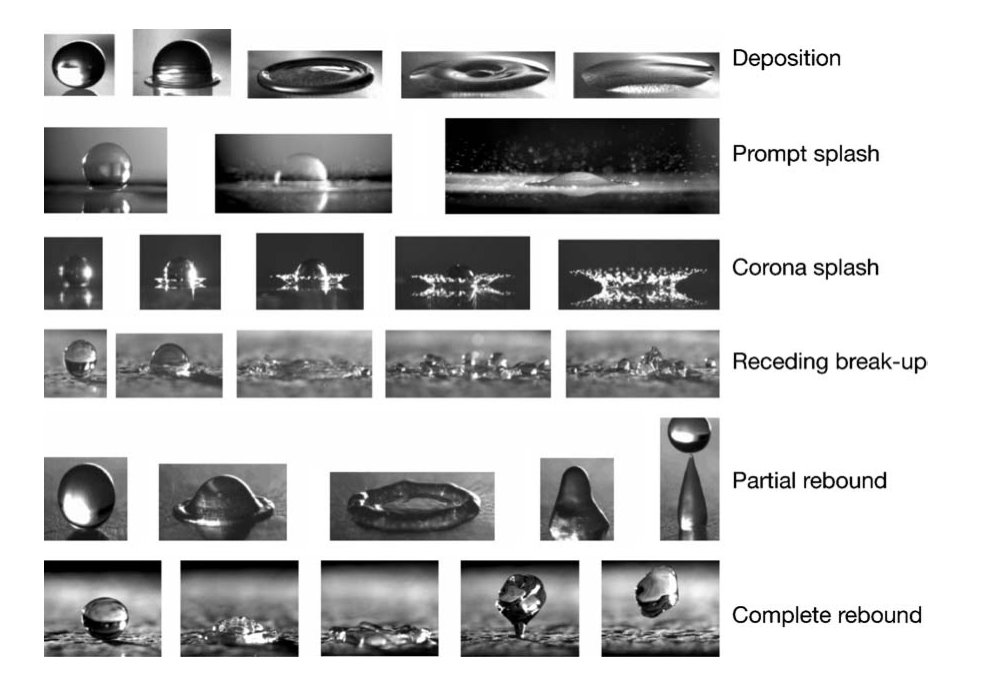
\includegraphics[scale=0.9]{rioboo.eps}
 \caption[Possible outcomes of droplet impact]{Six possible outcomes of droplet impact by \cite{Rioboo2001} }
 \label{rioboo}
\end{figure}
Many scientists have been interested in droplet impact on hydrophobic surfaces. In one such study \cite{Richard2002} found that the contact time of 
bouncing drop does not depend upon the impact velocity of the drop (See Figure \ref{richard2}).
\begin{figure}[tbp]
\centering
 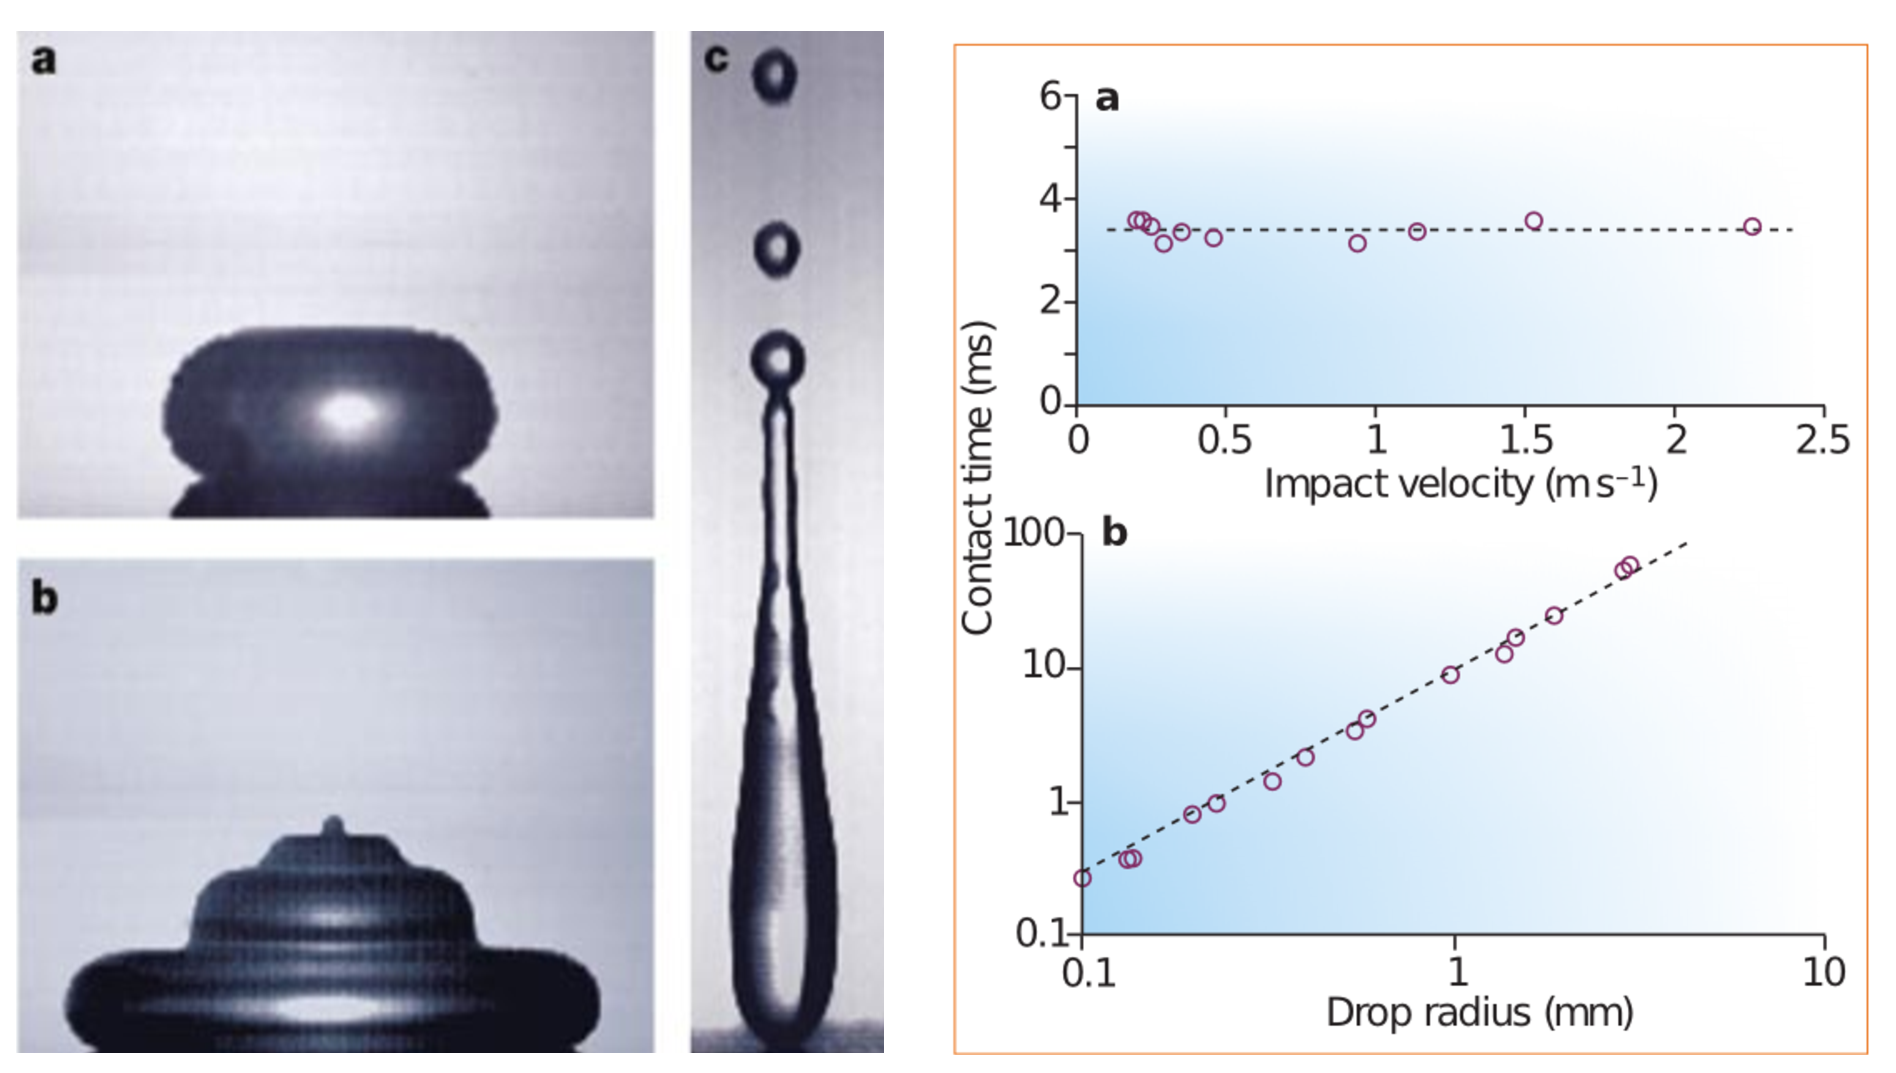
\includegraphics[scale=0.4]{richardc.eps}
 \caption[Contact time of droplet impact on hydrophobic surfaces ]{Contact time of droplet impact on hydrophobic surfaces by \cite{Richard2002} }
 \label{richard2}
\end{figure}
Movement of contact line is a complex phenomena which \cite{Roux2004} studied and obtained an empirical relationship with wetting velocity
of contact line and the impact velocity of the drop. This was later verified by \cite{Hung2011}.
There are a lot of studies on newtonian fluid droplet impact but \cite{Crooks2001} performed some experiments on non-newtonian 
fluids and concluded that the recoil behavior of droplet does not depend on the dynamic surface tension below a critical surfactant
concentration. Here surfactant was added to make the fluid non-newtonian.
\subsection{Simulations}
One of the very early simulation of droplet impact was by \cite{Harlow1967}. They solved the Navier-Stokes equations in cylindrical coordinates in order to
investigate the splash of a drop on a flat plate and deep pool. They used the Marker and Cell {(MAC)} method for interface tracking. The effect of microscopic 
factors such as molecules movement of fluid contact line and surface roughness were also verified by \cite{Gunjal2005} through simulations and experiments. Impact on
inclined surfaces have also received attention in past few years by \cite{Pasandideh1996}, \cite{Kang2000}, \cite{Fukai2000}, \cite{Bussmann1999} and \cite{Sikalo2005}.
These also have been studied by \cite{Lunkad2007} through simulations. \cite{Lunkad2007} applied a Dynamic Contact Angle {(DCA)} model and compared it with Static Contact 
Angle {(SCA)} results, and recommended   {(DCA)} for numerical simulations for better results.

\begin{figure}[tbp]
\centering
 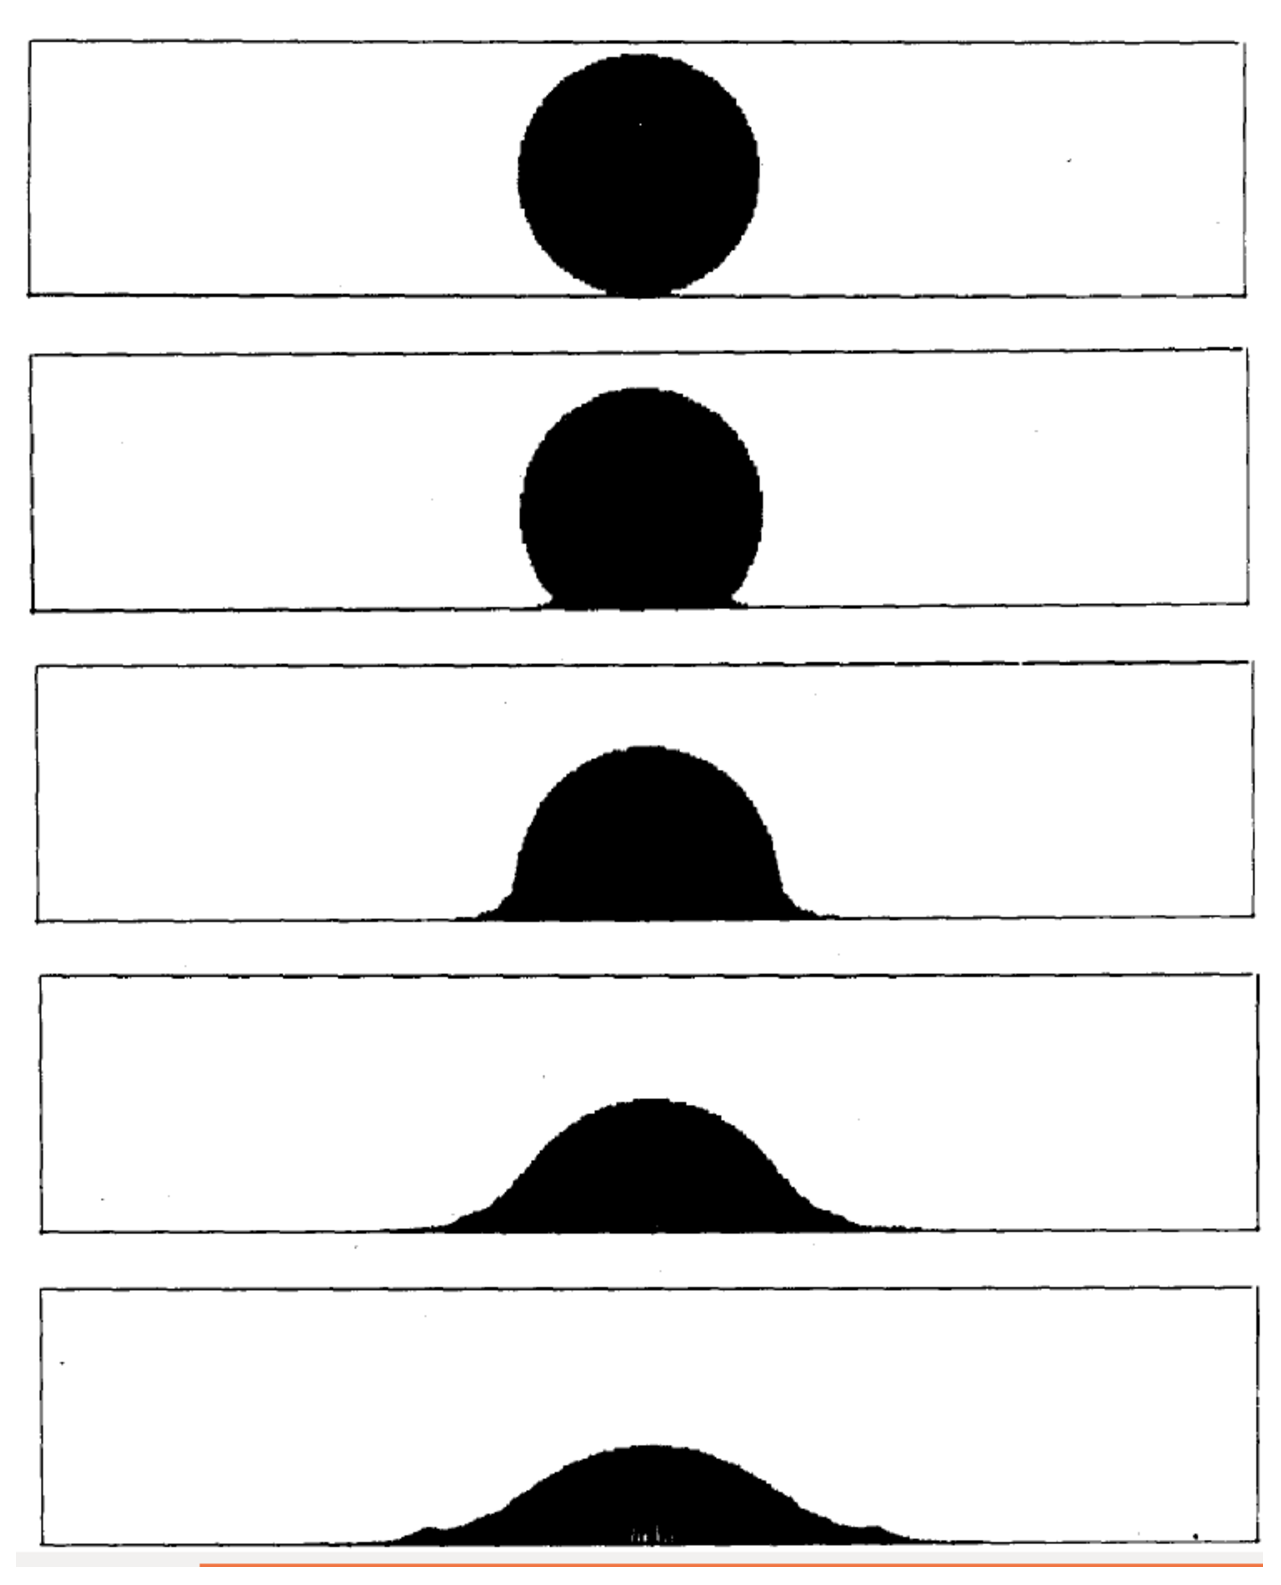
\includegraphics[scale=0.4]{harlow.eps}
 \caption[First numerical study on droplet impact]{The very first numerical study of droplet 
 impact (Reproduced by \cite{Harlow1967} under fair usage policy)}
\end{figure}

\subsection{Theory}
There have been many attempts to explain and model some phenomena which occurs during droplet impact such as 
spread of the droplet after impact. These have been investigated by \cite{Madejski1976}, \cite{Jones1971}, \cite{Chandra1991}, \cite{Scheller1995}, \cite{Bennett1993}, \cite{Pasandideh1996}.
A model was proposed by \cite{Mao1997} for maximum spread as a function of 
 Weber number, Reynolds number, and static contact angle. They also derived a model to predict the rebound by applying conservation of energy, as a function of 
 static contact angle and maximum spread diameter.
Recently a remarkable study by \cite {Liu2015} explained the splashing of droplet on smooth surfaces being due to Kelvin-Helmholtz instability in ultra-thin layer of 
air between the droplet and the surface (See Figure \ref{Fig:liu}).
\begin{figure}
 \centering
 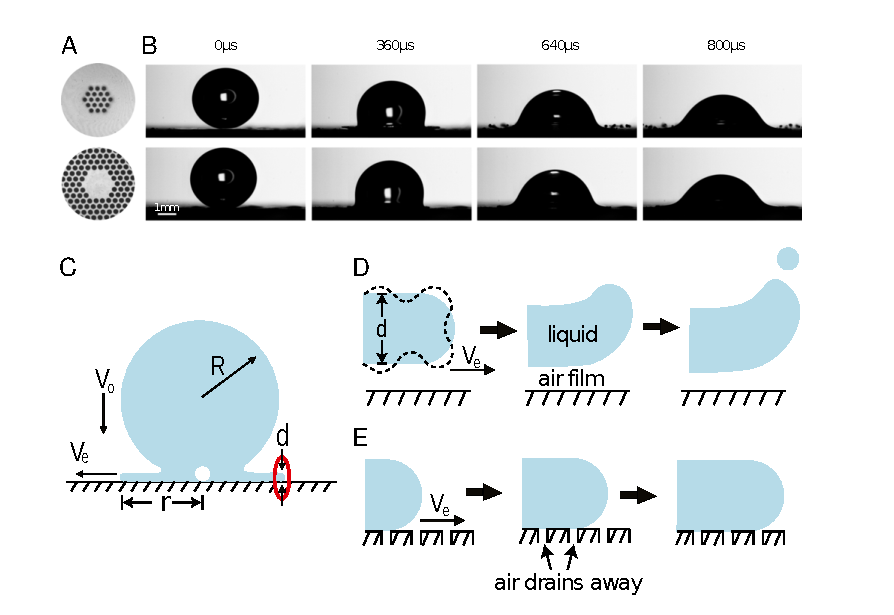
\includegraphics{Liu2015.eps}
 \caption[Kelvin-Helmholtz instability in a droplet splash]{Graphics verifying and explaining the KH instability in the droplet impact which initiates splash (Reproduced by \cite{Liu2015} under fair usage policy)}
 \label{Fig:liu}
\end{figure}

\section{Discussion}
The simulation droplet impact is a complex study as the multiphase solvers must take the effect of surface into the solution. The boundary conditions at the impact surface are non trivial. It
requires understanding of moving contact lines and dynamic contact angles which then has to be implemented in the numerical study. Droplet impact on superhydrophobic surfaces 
however are simpler to study because of the negligible effect of contact line.

